\section{Experiments}
\label{sec:experiments}

\begin{figure}[t]
    \centering
    \includegraphics[width=1\linewidth]{figures/random_forest_permutation_based_feature_importance.png}
    \caption{Top 20 features used by our \textsc{Random Forest} classifier determined by a permutation-based feature importance method \citep{breiman2001random}. Each feature is permuted 50 times.}
    \label{fig:random_forest}
\end{figure}

\begin{figure}[t]
    \centering
    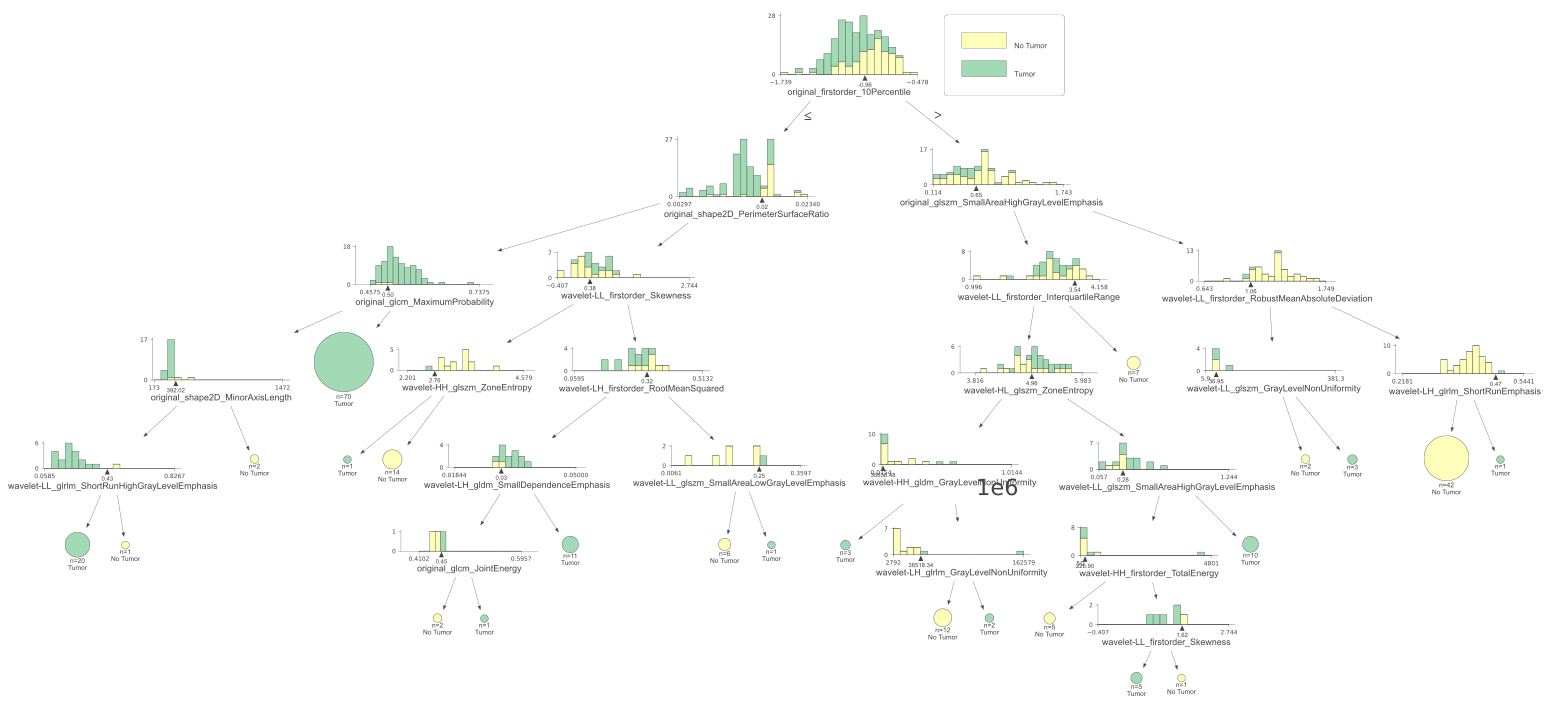
\includegraphics[width=1\linewidth]{figures/decision_tree}
    \caption{Visualization of our \textsc{Decision Tree} classifier. The visualization is generated using the \href{https://github.com/parrt/dtreeviz}{dtreeviz} library.}
    \label{fig:decision_tree}
\end{figure}

\begin{figure}[t]
    \centering
    \includegraphics[width=0.8\linewidth]{figures/logistic_regression_feature_importance.png}
    \caption{Absolute coefficients of our \textsc{Logistic Regression} classifier sorted by magnitude.}
    \label{fig:coeffslogreg}
\end{figure}  % write something about how only few parameters important and lasso regression forces parameters to 0

\begin{figure}[t]
    \centering
    \includegraphics[width=1\linewidth]{figures/logistic_regression_top20.png}
    \caption{Top 20 most important features of our \textsc{Logistic Regression} classifier and their corresponding coefficients.}
    \label{fig:top20logreg}
\end{figure}

\begin{figure*}
\centering
\begin{subfigure}{0.5\linewidth}
  \centering
    \includegraphics[width=1\linewidth]{figures/baseline_cnn_correct_shap.jpeg}
    \caption{}
    \label{fig:baseline_cnn_correct_shap}
\end{subfigure}%
\begin{subfigure}{0.5\linewidth}
  \centering
    \includegraphics[width=1\linewidth]{figures/transfer_learning_correct_shap.jpeg}
    \caption{}
    \label{fig:transfer_learning_correct_shap}
\end{subfigure}
\caption{SHAP images. (a) \textsc{Baseline CNN} (Actual: Tumor, Pred: Tumor). (b) \textsc{VGG16 TL} (Actual: Tumor, Pred: Tumor).}
\label{fig:shap}
\end{figure*}

\begin{figure}
\centering
\begin{subfigure}{.5\linewidth}
  \centering
    \includegraphics[width=0.9\linewidth]{figures/4__pred_0__label_0.png}
    \caption{}
    \label{fig:limenotumor}
\end{subfigure}%
\begin{subfigure}{.5\linewidth}
  \centering
    \includegraphics[width=0.9\linewidth]{figures/6__pred_1__label_1.png}
    \caption{}
    \label{fig:limetumor}
\end{subfigure}
\caption{\textsc{Baseline CNN} LIME explanations. (a) Actual: No Tumor, Pred: No Tumor. (b) Actual: Tumor, Pred: Tumor.}
\label{fig:lime}
\end{figure}
  % Write something about how looks at entire brain and no tumor visible
  % Write something about how tumor clearly marked and looked at by model


\subsection{Experimental Setup}
All of our experiments were performed on a 2021 MacBook Pro (Model Identifier MacbookPro18,3) with the Apple M1 Pro chip and 16 GB of memory running macOS Monterey 12.3.1.
We repeated every classical ML model run five times with consecutive seeds (seed 42 to 46) and report the mean and standard deviation. DL models were only run once using seed 0.

The tree-based models and the logistic regression classifier were developed using Scikit-learn \citep{scikit-learn}. We used PyTorch \citep{pytorch2019} to develop the CNN models and Tensorflow \citep{tensorflow2015-whitepaper} the VGG16 transfer learning model. The CNN models were trained with the Adam optimizer \citep{kingma2014adam} using a learning rate of $0.001$ and batch size of 64 for a maximum of 50 epochs using early stopping. Convergence was assumed when the cross-entropy loss did not improve on the validation set for 5 consecutive epochs. The VGG16 transfer learning model was also trained using the Adam optimizer but for 100 epochs with an exponentially decaying learning rate of $0.001$ and a batch size of 128. Again, we used early stopping but with a patience of 7 epochs. The final models are those with the lowest validation loss.

Hyperparameters were tuned on a hold-out validation set using extensive random searches \citep{bergstra2012random}. Optimal configurations can be found in the source code. Our final models were trained on the combined training and validation set to further increase performance.


\subsection{Results and Discussion}

\autoref{tab:results} shows the performance of our evaluated models on the the test sets. We observe that the more complex models show significantly better performance both in terms of accuracy and F1-score compared to the interpretable and simpler models. The VGG16 transfer learning model and pre-training on ImageNet, however, performed worse than our CNN baseline, likely due to the small size of our dataset and overfitting to the training and validation data. We also notice that the random forest classifier does not seem to improve upon the more interpretable decision tree on our dataset. Again, this is likely due to the small size of the dataset and overfitting.

We add several visualizations of our models to aid interpretability and explainability. In \autoref{fig:decision_tree} we visualize the splits of each node in the decision tree to explain its predictions. This visualization further suggests which features are important in classifying whether there are a visible brain tumors or not in the MRI images. In \autoref{fig:random_forest} we visualize the top 20 features used by our random forest classifier determined by a permutation-based feature importance method \citep{breiman2001random}. First-order wavelet features seem to be the most important in its predictions. Similarly, in \autoref{fig:coeffslogreg} and \autoref{fig:top20logreg} we visualize the most important features of our logistic regression classifier. Only $\sim100$ coefficients are non-zero and again first-order wavelet features seem play an important role in its predictions.

For our DL-based models, we visualize our post-hoc explanation methods in \autoref{fig:shap} and \autoref{fig:lime}. In \autoref{fig:baseline_cnn_correct_shap}, we can clearly see that our CNN model is focusing on the area within the brain that has a tumor according to the SHAP values and thus explaining the prediction. Similar patterns can be noticed in \autoref{fig:transfer_learning_correct_shap} for our VGG16 transfer learning model. Misclassifications and their corresponding SHAP values can be found in \autoref{sec:appendix_misclassified}. Lastly, in \autoref{fig:lime} we visualize the LIME explanations for our CNN baseline. Again, we can see that the model highlights the interesting regions, specifically we see that the entire tumor region is highlighted for the tumor prediction. The highlighted regions may be especially important in a clinical setting, where specialists are able to quickly verify the models' predictions by inspecting these regions.

Based on our visualizations as well as our models' performance, we recommend the \textsc{Baseline CNN} as the optimal classifier trading off interpretability for significantly increased performance. Both SHAP and LIME provide adequate explanations of the model's prediction and would help increase trustworthiness in a clinical setting even if CNNs are otherwise black boxes and offer very limited interpretability.
